\documentclass{article}
\usepackage[utf8]{inputenc}
\usepackage{setspace}
\usepackage{tikz}
\usetikzlibrary{positioning}
\usepackage{amsfonts}
\usepackage{amssymb}
\usepackage{amsmath}
\usepackage{amsthm}
\usepackage{systeme}
\usepackage{mathtools}
\usepackage{hyperref}
\usepackage{venndiagram}
\usepackage{pgfplots}
\usetikzlibrary{pgfplots.statistics}
\usetikzlibrary{arrows}
\pgfplotsset{compat=newest}

\allowdisplaybreaks

\begin{document}
\section*{Question 1}

~

\begin{proof}
    \begin{align*}
        &\text{Suppose }m>n\\
        &\left|x_{m}-x_{n}\right|\leqslant \sum_{i=n}^{m-1}|x_{i+1}-x_i|\\
        &\sum_{i=n}^{m-1}\left|x_{i+1}-x_i\right|\leqslant\sum_{i=n}^{m-1}2^{-i}\\
        &\sum_{i=n}^{m-1}2^{-i}=2^{-n}\left(\frac{1-2-2^{-(m-n)}}{1-2^{-1}}\right)=2^{-(n-1)}-2^{-(m+1)}<2^{-(n-1)}\\
        &\{2^{-n}\}_{n\to\infty}\to0\\
        \Rightarrow&\forall \varepsilon>,\exists n:0<2^{n}<2^{-(n-1)}<\varepsilon\\
        &N\coloneqq n-1\\
        \Rightarrow&m>n>N,\left|x_{m}-x_{n}\right|<2^{N}<\varepsilon\\
        &m,n,N\text{ are arbitrary}\\
        \Rightarrow&\forall \varepsilon>0,\exists N: \forall m,n>N\in \mathbb{N}:\left|x_{m}-x_{n}\right|<\varepsilon\\
        &(x_n)\text{ is cauchy}\\
    \end{align*}
\end{proof}

\newpage

\section*{Question 2}

~

\begin{proof}
    \begin{align*}
        &(S_k)\coloneqq\left(\sum_{i=0}^{k}\frac{x^n}{n!}\right)\\
        &\text{Suppose }p>q\\
        &\left|S_p-S_q\right|\\
        =&\left|\sum_{i=0}^{p}\frac{x^i}{i!}-\sum_{i=0}^{q}\frac{x^i}{i!}\right|\\
        =&\left|\sum_{i=q+1}^{p}\frac{x^i}{i!}\right|\\
        &\frac{\frac{x^{n+1}}{(n+1)!}}{\frac{x^n}{n!}}=\frac{x}{n+1}\\
        &\left\{\frac{x}{n+1}\right\}_{n\to\infty}\to0\\
        \rightarrow&\exists n\text{ large enough}:\forall m>0,\frac{x^n}{n!}>\frac{x^{m+n}}{(m+n)!}\\
        \Rightarrow&\exists N:\forall p>q>N,\left|\sum_{i=q+1}^{p}\frac{x^i}{i!}\right|<(p-q)\left|\frac{x^q}{q!}\right|\\
        &\left\{(p-q)\left|\frac{x^q}{q!}\right|\right\}_{q\to\infty}\to0\\
        \Rightarrow&\forall \varepsilon>0,\exists q\in\mathbb{N}:(p-q)\left|\frac{x^q}{q!}\right|<\varepsilon\\
        &p,q\text{ are arbitrary}\\
        \Rightarrow&\forall \varepsilon>0,\exists N\in\mathbb{N}:p>q\geqslant N,|S_p-S_q|<\varepsilon\\
        &x\text{ is arbitrary in this case}\\
        \Rightarrow&\sum_{i=0}^{k}\frac{x^n}{n!}\text{ is convergent for any }x\\
    \end{align*}
\end{proof}

\newpage

\section*{Question 3}

~

\subsection*{(a)}

~

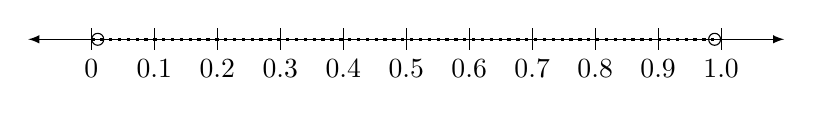
\begin{tikzpicture}[scale=8]
    \draw[latex-latex] (-0.1,0) -- (1.1,0) ; %edit here for the axis
    \foreach \x in  {0,0.1,0.2,0.3,0.4,0.5,0.6,0.7,0.8,0.9,1.0} % edit here for the vertical lines
    \draw[shift={(\x,0)},color=black] (0pt,0.5pt) -- (0pt,-0.5pt);
    \foreach \x in {0,0.1,0.2,0.3,0.4,0.5,0.6,0.7,0.8,0.9,1.0} % edit here for the numbers
    \draw[shift={(\x,0)},color=black] (0pt,0pt) -- (0pt,-0.5pt) node[below] 
    {$\x$};
    \draw[o-o] (0,0) -- (1,0);
    \draw[very thick,dotted] (0.0,0) -- (1,0);
\end{tikzpicture}

~

\subsection*{(b)}

~

\begin{proof}
    \begin{align*}
        &(S_n)\coloneqq\left(\frac{1}{2}+7\times10^{-(n+1)}\right)\\
        \Rightarrow&S\subseteq E\\
        &\left\{7\times10^{-(n+1)}\right\}_{n\to\infty}\to0\\
        \Rightarrow&\lim_{n\to\infty}7\times10^{-(n+1)}=0\\
        &\lim_{n\to\infty}\frac{1}{2}+7\times10^{-(n+1)}=\frac{1}{2}\\
        &\forall n,\frac{1}{2}\ne S_n\\
        \Rightarrow&\frac{1}{2}\text{ is a cluster point of }E\\
    \end{align*}
\end{proof}

\newpage

\section*{Question 4}

~

\begin{proof}
    \begin{align*}
        &\delta:0<|x+1|<\delta \\
        &\left|\frac{x^4-2x^3+x^2-1}{3x^6+x^3+1}-1\right|\\
        =&\left|\frac{-3x^6+x^4-3x^3+x^2-2}{3x^6+x^3+1}\right|\\
        =&\left|\frac{(x+1)(-3x^5+3x^4-2x^3-x^2+2x-2)}{3x^6+x^3+1}\right|\\
        =&\left|x+1\right|\left|\frac{-3x^5+3x^4-2x^3-x^2+2x-2}{3x^6+x^3+1}\right|\\
        &\text{set }|x+1|<\frac{1}{10}\\
        \Rightarrow&x\in(-1.1,-0.9)\\
        \Rightarrow&\frac{-3x^5+3x^4-2x^3-x^2+2x-2}{3x^6+x^3+1}<1.3\\
        &\left|x+1\right|\left|\frac{-3x^5+3x^4-2x^3-x^2+2x-2}{3x^6+x^3+1}\right|<1.3|x+1|\\
        &\varepsilon>0,\delta\coloneqq \min\left\{\frac{1}{10},\frac{\varepsilon}{1.3}\right\}\\
        \Rightarrow&\forall \varepsilon>0,\exists \delta>0:0<|x+1|<\delta\implies \left|\frac{x^4-2x^3+x^2-1}{3x^6+x^3+1}-1\right|<\varepsilon\\
    \end{align*}
\end{proof}
\end{document}

